% !TEX root = main.tex
\documentclass[a4paper, UKenglish, 11pt]{uiomaster}
\usepackage{lipsum}
\usepackage[subpreambles=true]{standalone}
\usepackage[table,xcdraw]{xcolor}
\usepackage{graphicx}




% MSE as loss function
% Training and testing, lr ?

\begin{document}
\chapter{Training the Fully Connected Feed-Forward Neural Network} \label{chap:training_FCNN}
\chaptermark{Training the FCNN}

This chapter will explore the training process of the fully connected feed-forward neural network (FCNN), outlining the decisions made. Carefully choosing and adjusting elements of the training process ensures the FCNN's ability to make accurate predictions, establishing it as a valuable tool for solving the inverse EEG problem. Subsequent chapters will delve into the results and outcomes of this training, providing insights into the model's effectiveness.

\section{Overview of Training Methods}
Having constructed the fully connected feed-forward neural network architecture, we now embark on the phase of training the model to effectively localize current dipoles from EEG signals. This chapter delves into the process of training the FCNN and addresses various aspects that influence the performance of the network. Training a neural network requires careful consideration and tuning of several key factors to achieve optimal results. In the process of training FCNN, we will explore the following essential elements:

\begin{description}
   \item [Data Preparation:] We begin by preparing the data set, involving data segmentation and standardization.

   \item [Cost Function:] Moving forward, we explore the significance of the cost function in guiding the network towards convergence. Understanding how to choose the appropriate cost function tailored to the problem is important.

   \item[Backpropagation:] The backpropagation algorithm is used to calculate the gradients of the cost function with respect to the trainable parameters of the model.

   \item[Optimization Algorithm:] The gradients calculated during backpropagation are used to update the values of the parameters of the model in order to minimize the cost. The choice of optimization algorithm plays an important role in training efficiency and convergence speed. We delve into the technique of gradient descent and its implications in the context of the FCNN.

   \item[Regularization Techniques:] Overfitting is a common challenge in neural network training. We examine regularization techniques like dropout and weight decay to mitigate this issue.

   \item[Learning Rate Scheduling:] Finally we present the method of adaptive learning rates. We discuss how learning rates significantly influence training dynamics, and how methods for scheduling learning rates during training ensure steady convergence.

\end{description}





\section{Data Preparation}

\subsection{Data Segmentation}

The first step in preparing to \emph{fit} a machine learning model, is to perform a split of the data set $\mathcal{D}$ into distinct sets for training, validation, and testing. As the name suggests, training data is used for training the model, while validation and test data are used for evaluating the model's performance on unseen samples. This allows us to check for and avoid \emph{overfitting}, a phenomenon where the network becomes excessively attuned to the training data and consequently performs poorly on new data.
The size of each set commonly depends on the size of the data set available, however a general guideline is that the majority of the data are allocated into the training set with the remainder going into the validation and test sets \cite{mehta2019high}.

The data set of simulated EEG signals contains 70,000 samples. 20,000 of these are randomly selected for the test set. Of the remaining 50,000 samples, 80 percent are randomly assigned to the training set with the rest making up the validation set.
Upon completion of the training process, the test set serves as the ultimate benchmark for evaluating the model's capacity to generalize and make accurate predictions on new instances of data. By adhering to this train-validation-test data partitioning, we ensure a robust evaluation of the FCNN's performance and its capacity to effectively handle real-world scenarios with previously unseen data.



\subsection{Data Scaling}

Having addressed the data segmentation, we proceed to the task of \emph{data scaling}, which is a highly recommended procedure within machine learning. \emph{Data standardization} involves centering the EEG data of the design matrix \(X\) around the mean and scaling it to achieve unit standard deviation. To achieve this we calculate the mean \(\mu\) and the standard deviation $\sigma$ of all the elements in \(X\). We then subtract \(\mu\) from \(X\) element-wise and divide by \(\sigma\),
\begin{equation}
  X' = \frac{X - \mu}{\sigma},
\end{equation}
to produce a scaled design matrix with zero mean and unit standard deviation.





\section{Cost Function}

In the field of machine learning, \emph{cost functions} are used to evaluate how well models make predictions.
Selecting an appropriate cost function is important. In our regression task, where the objective is to predict $x$, $y$, and $z$ coordinates of single current dipoles, we use Euclidean distance to quantify the error of a single sample. For a batch of \(N\) samples we use mean Euclidean distance, defined by
\begin{equation}
  \text{MED}(\boldsymbol{\theta})
    = \frac{1}{N} \sum_{i=1}^{N}
        \sqrt{(x_i - \tilde{x}_i)^2 + (y_i - \tilde{y}_i)^2 + (z_i - \tilde{z}_i)^2}.
  \label{eq:MED}
\end{equation}
Here $\boldsymbol{\theta}$ are the model parameters,
\(x_i, y_i, z_i\)
denote the predicted values, and $\tilde{x}_i, \tilde{y}_i, \tilde{z}_i$ are the corresponding true values.

\begin{note}
  Due to the squaring step in the function, which penalizes larger errors more severely, the trained model is less likely to generate outlier predictions with substantial errors. However, in situations where the model produces a single, highly inaccurate prediction, the squaring effect can significantly amplify the error. Nevertheless, in many practical scenarios, the primary focus is not on these individual outliers, but rather on achieving a well-balanced model that delivers satisfactory performance across the majority of predictions \cite{builtin-ml-loss-functions}.

  In our simulation-driven context, devised to accommodate a spectrum of diverse EEG variations, it is noteworthy that the presence of apparent outliers is not rooted in sampling errors, but rather random fluctuations and indicative of distinct scenarios. As delineated in statistical literature \cite{barnett1994outliers}, an outlier is characterized as an observation that seemingly deviates from the prevailing distribution of a data set. This departure can be attributed to human or instrumental anomalies in the data acquisition process \cite{zhang2015outlier}. Figure \ref{fig:outliers} vividly depicts the distribution of minimum and maximum EEG observations across individual samples within the data set. While the majority of data points exhibit values within the range of -1.5 to 3 $\mu$V, a subset extends beyond these bounds. It is crucial to underscore that these data points do not emerge as stochastic errors stemming from the acquisition process. Instead, they intentionally embody distinctive EEG signals that enrich the data set's representational fidelity within authentic real-world contexts.
\end{note}





\section{Backpropagation Algorithm}

The backpropagation algorithm is a fundamental technique used in neural networks in order to adjust the weights for the purpose of minimizing the cost function. To explain the implementation details of this technique, we follow the guidance provided in the book \textit{A high-bias, low-variance introduction to machine learning for physicists} (Pankaj Mehta, et al., 2019) as it offers a comprehensive treatment of the topic. The backpropagation technique leverages the chain rule from calculus to compute gradients for weight adjustments and can be summarized using four equations.

Before introducing the equations, Mehta et al. establish some useful notation. We let $L$ denote the total number of layers within the neural network, with each layer identified by an index $l$ ranging from 1 to $L$ inclusive. Like in Chapter \ref{chap:fcnn-approach} the weights of layer \(l\) are denoted $w^{(l)}_{ik}$. They represent the strength of the connection between the $k$-th neuron in the previous layer, $l-1$, and the $i$-th neuron in the current layer, $l$. The bias of node \(i\) in layer \(l\) is denoted $b^{(l)}_i$.

The first of the four equations is the shorthand
\begin{equation}
  \delta_i^{(l)} = \frac{\partial C}{\partial z_i^{(l)}},
  \label{eq:I}
\end{equation}
where
\begin{equation}
  z_i^{(l)} = \sum_{j = 1}^{N_{l - 1}} w_{i j}^{(l)} a_j^{(l - 1)} + b_i^{(l)}
  \label{eq:z_i}
\end{equation}
is the value of the \(i\)-th neuron in layer \(l\) pre-activation.
The quantity \(\delta_i^{(l)}\) can be thought of as the change to the cost function caused by an infinitesimal increase in $a_i^{(l)}$.

The partial derivative of the cost function with respect to the bias $b_i^{(l)}$ is \(\delta_i^{(l)}\):
\begin{equation}
  \frac{\partial C}{\partial b_i^{(l)}}
    = \frac{\partial C}{\partial z_i^{(l)}} \frac{\partial z_i^{(l)}}{\partial b_i^{(l)}}
    = \delta_i^{(l)}.
  \label{eq:II}
\end{equation}
When applying the chain rule here, we have used the fact that the \(i\)-th node in the \(l\)-th layer is the only one whose activation is influenced by \(b_i^{(l)}\).

By applying the chain rule, we can express the error $\delta_i^{(l)}$ in Equation \ref{eq:I} in terms of the equations for layer $l+1$, giving us the third equation used in the backpropagation algorithm:
\begin{align}
  \delta_i^{(l)} = \frac{\partial C}{\partial z_i^{(l)}}
    &= \sum_{j = 1}^{N_{l + 1}} \frac{\partial C}{\partial z_j^{(l+1)}} \frac{\partial z_j^{(l+1)}}{\partial z_i^l} \nonumber \\
    &= \sum_{j = 1}^{N_{l + 1}} \delta_j^{(l+1)}
      \frac{\partial z_j^{(l+1)}}{\partial a_i^{(l)}}
      \frac{\partial a_i^{(l)}}{\partial z_i^{(l)}} \nonumber \\
    &= \sum_{j = 1}^{N_{l + 1}} \delta_j^{(l+1)} w_{ji}^{(l+1)}
      \left. \frac{\partial \text{ act}^{(l)}(z)}{\partial z} \right|_{z_i^{(l)}}. \label{eq:III}
\end{align}
The last factor in the last line is the derivative of the activation function in the \(l\)-th layer evaluated at \(z_i^{(l)}\).

Finally the last of the four backpropagation equations is the derivative of the cost function with respect to the weights:
\begin{equation}
  \frac{\partial C}{\partial w_{ij}^{(l)}}
    = \sum_{k = 1}^{N_l} \frac{\partial C}{\partial z_k^{(l)}} \frac{z_k^{(l)}}{\partial w_{ij}^{(l)}}
    = \delta_i^{(l)} a_j^{(l-1)}.
\label{eq:IV}
\end{equation}

With these four equations in hand we can calculate the gradient of the cost function with respect to all the weights and biases of the network starting from the output layer and working our way backwards. The backpropagation algorithm can be performed with the four following steps:
1) Do a forward pass calculating \(z_i^{(l)}\) and \(a_i^{(l)}\) for all layers.
2) Calculate the cost of the prediction.
3) Propagate the error backwards and calculate $\delta_j^{(l)}$ for all layers, using equation \ref{eq:III}.
4) Use equation \ref{eq:II} and \ref{eq:IV} in order to calculate
$\frac{\partial C}{\partial b^{(l)}_{i}}$
and
$\frac{\partial C}{\partial w^{(l)}_{ij}}$.

This description makes clear the incredible utility and computational efficiency of the backpropagation algorithm. Derivatives can be calculated using so-called “forward” and “backward” passes through the neural network. This offers computational efficiency which is essential when having to calculate the gradient with respect to all parameters of the neural network at each step of \emph{gradient descent}, an optimization algorithm that we will be delving into in the next section.

\rednote{Autograd in PyTorch \dots}





\section{Optimization Algorithm}

\subsection{Gradient Descent}

\rednote{Doublecheck citing.}
In order to minimize the cost function and find the optimal values for the model parameters, $\boldsymbol{\theta}$, an optimization algorithm is employed. One widely used optimization algorithm is \emph{gradient descent}, which iteratively updates the parameters based on the gradient of the cost function with respect to the parameters \cite{mehta2019high}.

Gradient descent is an iterative optimization algorithm used to locate a local minima of a differentiable function. The core concept of the algorithm is based on the observation that a function $F(\textbf{x})$ will decrease most rapidly if we repeatedly move in the opposite direction of the gradient of the function, i.e. in the direction of
$- \nabla F(\textbf{x})$. This means that the sequence
\(\{\textbf x_0, \textbf x_1, \dots \}\)
given by
\begin{equation}
  \label{eq:gradient-descent-general-sequence}
  \textbf{x}_{n+1} = \textbf{x}_n - \eta \nabla F(\textbf{x}_n)
\end{equation}
for a sufficiently small \emph{learning rate} $\eta$ will consist of points at which the function \(F\) has smaller and smaller values.
The process begins with an arbitrary initial point $\textbf x_0$, and eventually converges to a local minimum of \(F\).

In the neural network weights and biases are updated as follows to find a minimum of the cost function \(C\):
\begin{align}
  w_{ij}^{(l)} &\to w_{ij}^{(l)} - \eta \frac{\partial C}{\partial w_{ij}^{(l)}} \\
  b_i^{(l)} &\to b_i^{(l)} - \eta \frac{\partial C}{\partial b_i^{(l)}}.
\end{align}

It is important to note that the error function in gradient descent is computed based on the entire training set, meaning that all samples are processed in order to evaluate the gradient in every step, which is often inefficient. Another potential issue with gradient descent is its sensitivity to the initial values of the model parameters, and the choice of the learning rate $\eta$. The sensitivity to initial conditions can be explained by the fact that we often deal with high-dimensional, non-convex cost functions with numerous local minima where we risk getting stuck in a suboptimal region of the parameter space. Choosing a too large learning rate may result in overshooting minima, leading to unpredictable behavior, while a too small learning rate increases the number of iterations required to reach a minimum. Stochastic Gradient Descent, described in the next subsection, is a popular alternative which attempts to mitigate some of these issues \cite{bishop2006pattern}.



\subsection{Stochastic Gradient Descent}

The Stochastic Gradient Descent (SGD) method is a powerful optimization technique that diverges from traditional gradient descent by randomly selecting subsets of the data, called \emph{mini-batches}, during each iteration, as opposed to considering the entire data set \cite{bishop2006pattern}. This is also the main property that distinguishes it from traditional gradient descent. SGD restricts its focus to smaller portions of the data, meaning that only a subset of the data are processed when evaluating the gradient in each step.
This is efficient, as there is less computation required for each step in the gradient descent.

The random sampling of smaller subsets from the data introduces stochasticity to the model. This is a potential downside which could mean that the gradient calculated in one step does not point in the direction which minimizes the cost on the entire data set, which is what we ultimately want to do. However, this can potentially have a positive effect as well by allowing the model to escape a suboptimal local minima thanks to the small randomness introduced, which might allow the model to find superior solutions compared to gradient descent.



\subsection{Momentum}

Furthermore, an incorporation of \emph{momentum} into the SGD algorithm may enhance convergence speed even further. Momentum introduces a form of memory into the optimization process by accumulating information about previous movements in parameter space. Returning to our general description of gradient descent as a sequence of points which minimizes a function
\(F(\textbf x)\),
we update the procedure described by Equation
\eqref{eq:gradient-descent-general-sequence}
to
\begin{align}
  \textbf{v}_t &= \gamma \textbf{v}_{t-1} + \eta \nabla F(\textbf{x}_t), \\
  \textbf{x}_t &= \textbf{x}_{t-1} - \textbf{v}_{t}.
\end{align}
In these equations, $\textbf{v}_t$ represents the momentum vector at iteration $t$, $\gamma$ is the momentum coefficient, $\eta$ is the learning rate, and $\nabla F(\textbf{x}_t)$ signifies the gradient of $F_n$ \cite{Hjorth-Jensen2022}.

In our FCNN, these equations are used to update the weights and biases based on the gradients calculated during backpropagation using a separate momentum for each parameter.

During the training of the FCNN, we observed that a learning rate of 0.001 yielded the most favorable results. Moreover, a mini-batch size of 32 was employed. The momentum coefficient $\gamma$ was set to 0.35, a value that struck an optimal balance between convergence speed and sensitivity to the initial learning rate parameter.





% This approach is particularly beneficial when dealing with extensive data sets. The update step in SGD can be expressed as:
%
% \begin{equation}
% \textbf{w}{\tau+1} = \textbf{w}{\tau} - \eta\nabla F_n(\textbf{w}_\tau)
% \end{equation}
%
% Here, $\textbf{w}{\tau}$ represents the weight vector at iteration $\tau$, $\eta$ is the learning rate, and $\nabla F_n(\textbf{w}{\tau})$ is the gradient of the cost function $F_n$ computed on a mini-batch, which refers to a randomly selected subset of the complete data set.
%
% In essence, SGD mirrors regular gradient descent but restricts its focus to a single mini-batch at each iteration.



% The method of Stochastic Gradient Descent (SGD) allows us to compute the gradient by randomly selecting subsets of the data at each iteration, rather than using the entire data set \cite{bishop2006pattern}. The update can be written as:
%
% \begin{equation}
% \textbf{w}_{\tau+1} = \textbf{w}_{\tau} - \eta\nabla F_n(\textbf{w}_\tau)
% \end{equation}
%
% These smaller subsets taken from the entire data set are commonly reffered to as mini-batches. In other words, SGD is just like regular GD, except it only looks at one mini-batch for each step. Introducing fluctuation by only taking the gradient on a subset of the data, is beneficial as it enables the algorithm to jump to a new and potentially better local minima, rather that getting stuck in a local minimum point.
%
% Morover, adding \emph{momentum}, to the algorithm, leads to faster converging, due to stronger acceleration of the gradient vectors in the relevant directions, and also improves the algorithms sensitivity to initial guess of the learning rate $\eta$. The momentum can be understood as a memory of the direction of the movement in parameter space, which is done by adding a fraction $\gamma$ of the weight vector of the past time step to the current weight vector:
%
% \begin{equation}
% \textbf{v}_{\tau} = \gamma\textbf{v}_{\tau-1} - \eta\nabla F_n(\textbf{w}_{\tau})
% \end{equation}
%
% \begin{equation}
% \textbf{w}_{\tau} = \textbf{w}_{\tau-1} + \textbf{v}_{\tau}
% \end{equation}
%
% Here, $\textbf{w}{\tau}$ represents the updated weight vector at iteration $\tau$, $\textbf{w}_{\tau-1}$ is the previous weight vector, $\textbf{v}_{\tau}$ is the updated momentum vector at iteration $\tau$, $\gamma$ is the momentum coefficient, $\eta$ is the learning rate, and $\nabla F_n(\textbf{w}_{\tau})$ is the gradient of the cost function $F_n$ computed on the mini-batch.
%
% A learning rate of 0.001 proved the best when training DiLoc. Moreover a mini-batch size of 32 were utialized. The momentum hold a value of 0.35.





\section{Regularization Techniques}
% weight decay L2 pentalty
% dropout
Regularization techniques in machine learning help prevent overfitting. One common regularization technique is called the L2-norm penalty. In this technique, we add an extra term to our cost function that depends on the size of the model's weights. This added term ensures that the weights do not become excessively large while fitting the training data. By doing this, regularization reduces the risk of the model fitting the training data too closely, which can lead to overfitting. \cite{Hjorth-Jensen2022}.

We can measure the size of the weights using the L2-norm, which modifies our cost function from
\(C(\boldsymbol \theta)\)
to
\begin{equation}
  C'(\boldsymbol \theta)
    = C(\boldsymbol \theta) + \lambda\sum_{i,j,l} \left( w_{ij}^{(l)} \right)^2.
  \label{eq:L2}
\end{equation}
The tuning parameter $\lambda$ controls how much we penalize the flexibility of our model. Here, flexibility means how much the model can adjust its coefficients to fit the data precisely. Choosing a large value for $\lambda$ restricts the parameters to smaller values, giving a less flexible model which will try to find simpler patterns in the data, which in turn reduces the chances of overfitting \cite{gupta2017regularization}.





\section{Learning Rate Scheduling}

The learning rate \(\eta\) plays a critical role in the iterative Stochastic Gradient Descent procedure used to update model parameters during training, influencing the size of the steps taken to minimize the cost function. To simplify the process of selecting an appropriate learning rate we employ a \emph{learning rate scheduler}. This scheduler dynamically adjusts the learning rate during the optimization, enhancing both performance and training efficiency.

Various methods can be used to make the learning rate adaptive. A common approach involves starting with a higher learning rate at the beginning of training. This allows for larger steps during the initial phases, speeding up process. As training progresses and the model approaches convergence, smaller steps are taken to fine-tune the parameters near the minimum, preventing overshooting. This strategy balances rapid initial convergence with meticulous fine-tuning later on \cite{pytorch_learning_rate_schedule}.

We have used the PyTorch's built-in \texttt{ReduceLROnPlateau} \footnote{\url{https://pytorch.org/docs/stable/generated/torch.optim.lr_scheduler.ReduceLROnPlateau.html}}. This learning rate scheduler adjusts the learning rate when the change in the loss has been under a specific threshold for a certain number of epochs. In other words, the learning rate remains unchanged as long as it enhances model performance but is reduced when results starts converging.





% \section{Method that not belong here, but rather for the extended problems}


% The objective during training is to find the optimal parameters $\beta$ that minimize the cost function. The cost function represents the discrepancy between the network's predictions and the actual target values. By iteratively updating the parameters to minimize the cost function, the network fine-tunes its internal representations to make more accurate predictions. MSE is chosen as the cost function for the DiLoc network, as it provides a smooth and continuous measure of the model's performance during training, penalizing larger errors more heavily.
%
% % Include why we went for batch size 32 and mom = 0.35 (instead of 0.9)
% Optimizers play a crucial role in reducing the network's loss and providing accurate results. In this case, SGD with momentum is utilized as the network's optimizer. SGD with momentum enhances the sensitivity of the network to initialized weights and provides fast convergence. The algorithm uses mini-batches of size 32, introducing fluctuation to the data and preventing the network from getting stuck in local minima or saddle points. The momentum hyperparameter, set to 0.35 in this context, helps reduce high variances in the optimization process and accelerates convergence towards the right direction, leading to faster training.
%
%
%
% Additionally, L1 and L2 regularization techniques are incorporated as optional parameters into the DiLoc network. These regularization methods help prevent overfitting and improve generalization to unseen data. By adding penalty terms to the cost function, L1 and L2 regularization encourage the model to favor simpler and more generalizable solutions.
%
% After the DiLoc network is fully trained on the training data set, it has learned the optimal parameters to make accurate predictions. The model's performance is evaluated using a separate test data set, which the network has not seen during training. This test data provides an unbiased assessment of the model's accuracy and its generalization capabilities to unseen data.
%
% In the upcoming chapters, we will present different approaches to the inverse problem and showcase the performance of the DiLoc network across these approaches. The evaluation results will demonstrate the effectiveness and utility of the trained model in solving the localization task for various scenarios.




%
% \subsection{Choosing an Optimal Cost Function}
% % Include data distribution (min/max)
% In the field of machine learning, \emph{cost functions} play a crucial role in evaluating how well models make predictions. These mathematical functions compare predicted outcomes to actual values, resulting in a quantifiable metric known as \emph{loss}. Higher loss values indicate poorer model performance, while lower values reflect more accurate predictions.
%
% Selecting the appropriate cost function is pivotal in addressing machine learning challenges. In regression tasks like ours, the mean squared error (MSE) is a widely used cost function, particularly suitable for linear regression. The MSE is preferred due to its simplicity and continuous measure of model performance during training. It calculates the squared differences between the model's predictions and target values, then takes the mean across the entire data set:
%
% \begin{equation}
% \text{MSE}(\boldsymbol{\theta}) = \frac{1}{N-1}
% \sum_{i=0}^{N}(y_i-\tilde{y}_i)^2 ,
% \label{eq:MSE}
% %MSE(\textbf{y},\mathbf{\tilde{y}}) =
% \end{equation}
%
% Here $\boldsymbol{\theta} = \theta_0, \theta_1, ..., \theta_n$ represents the model parametes, $y_i$ stands for the predicted value and $\tilde{y}_i$ is the corresponding true value.
%
% Due to the squaring step in the MSE function, which penalizes larger errors more severely, the trained model is less likely to generate outlier predictions with substantial errors. However, in situations where the model produces a single, highly inaccurate prediction, the squaring effect can significantly amplify the error. Nevertheless, in many practical scenarios, the primary focus is not on these individual outliers, but rather on achieving a well-balanced model that delivers satisfactory performance across the majority of predictions \cite{builtin-ml-loss-functions}.
%
% % include how we do this in our thesis.
%
% In our simulation-driven context, devised to accommodate a spectrum of diverse variations, it's noteworthy that the presence of apparent outliers is not rooted in random fluctuations, but rather indicative of distinct scenarios. As delineated in statistical literature \cite{barnett1994outliers}, an outlier is characterized as an observation that seemingly deviates from the prevailing distribution of a data set. This departure can be attributed to human or instrumental anomalies in the data acquisition process \cite{zhang2015outlier}. Figure \ref{fig:outliers} vividly depicts the distribution of minimum and maximum EEG observations across individual samples within the data set. While the majority of data points exhibit values within the range of -1.5 to 3 $\mu$V, a subset extends beyond these bounds. It's crucial to underscore that these data points don't emerge as stochastic errors stemming from the acquisition process. Instead, they intentionally embody distinctive EEG signals that enrich the data set's representational fidelity within authentic real-world contexts.
%
% \begin{figure}[!htb]
%     \centering
%     \begin{subfigure}[b]{0.45\linewidth}
%         \centering
%         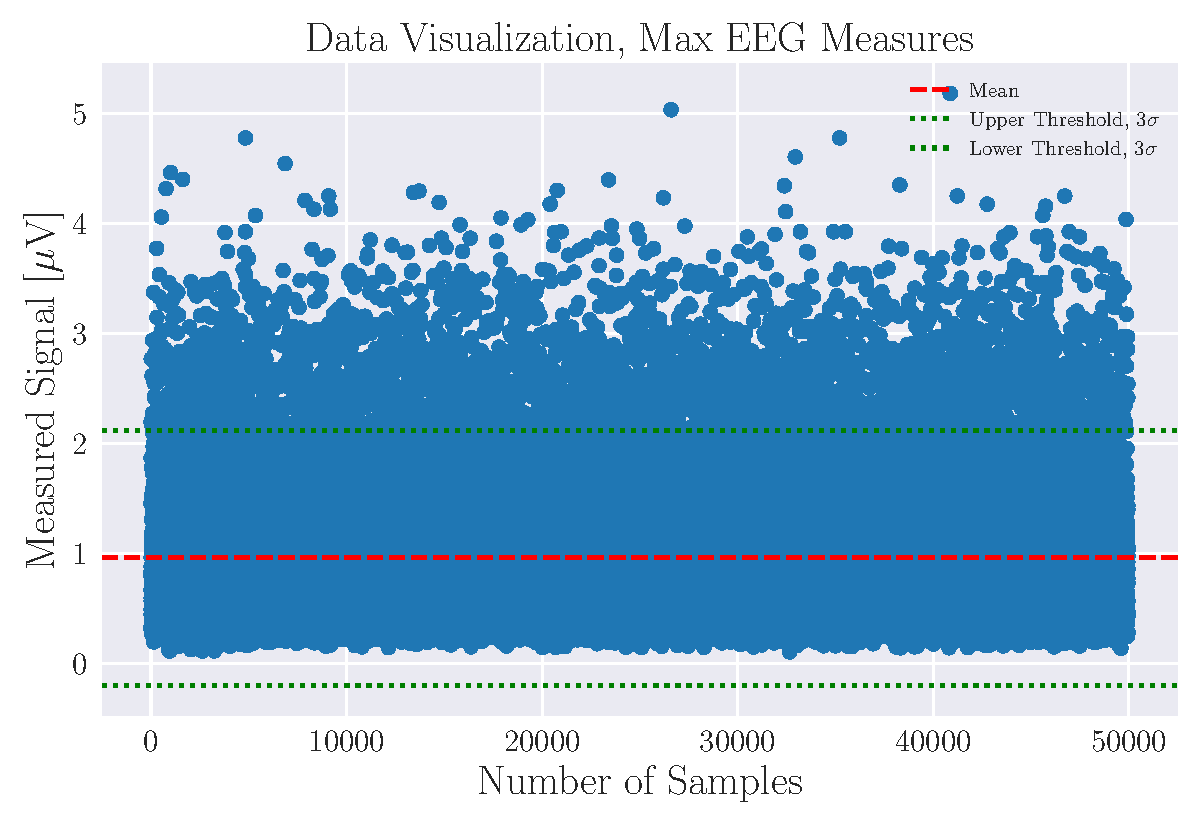
\includegraphics[width=\linewidth]{figures/data_visualization_max.pdf}
%     \end{subfigure}
%     \hfill
%     \begin{subfigure}[b]{0.45\linewidth}
%         \centering
%         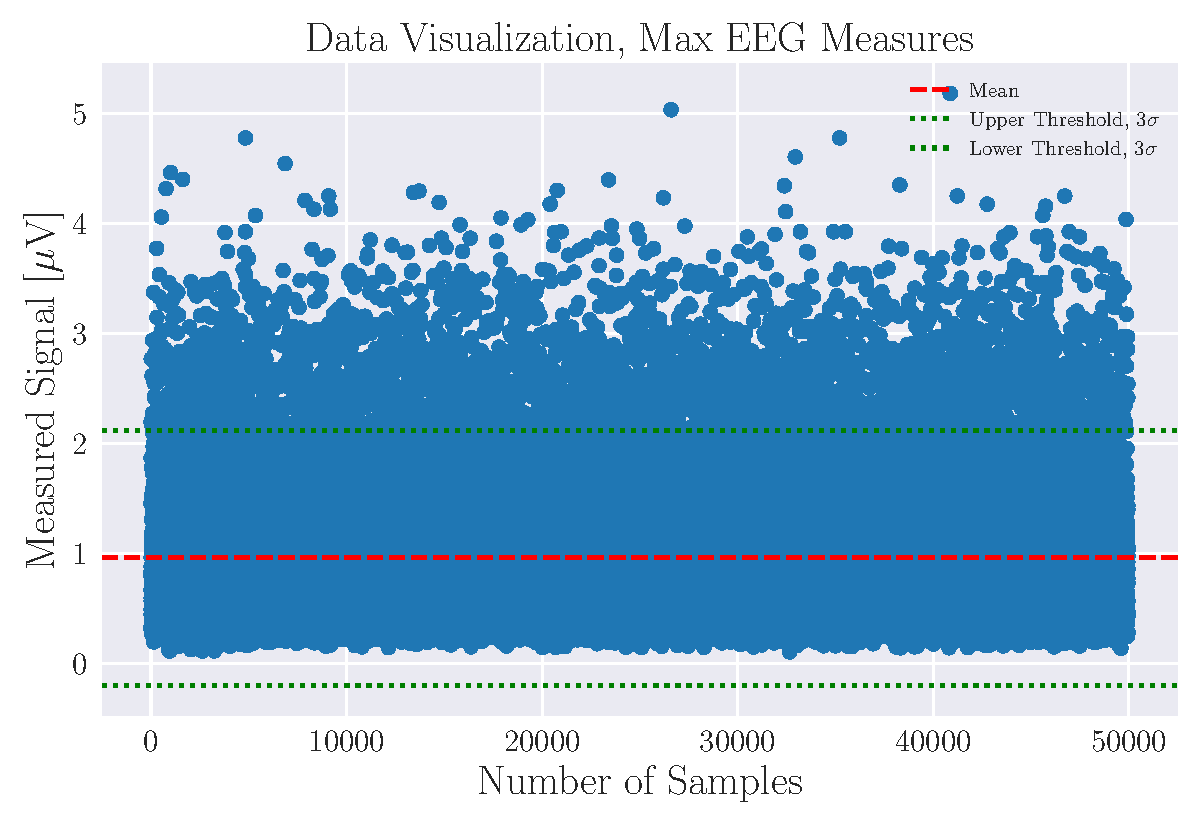
\includegraphics[width=\linewidth]{figures/data_visualization_max.pdf}
%     \end{subfigure}
%     \caption{\textbf{Visualization of data set.} Both panels visualize the maximum EEG measures for each sample within the data set.}
%     \label{fig:outliers}
% \end{figure}
%
% When having clear understandings of desired model outcomes, customized cost functions, designed to align precisely with specific objectives may potentially outperform the MSE cost function. Our objective is to create a model that first of all is capable of accurately predicting single dipole posistions, and as extensions also multiple dipole positions, amplitudes of dipole signals and radii of extended dipole populations.  To achieve this, the ideal cost function should minimize the Euclidean distance between target dipole localizations ${\theta}_{x,y,z}$ and true values $\tilde{\theta}_{x,y,z}$:
%
% \begin{equation}
%     \text{MED}_{\text{x,y,z}}(\boldsymbol{\theta}) = \frac{1}{n}\sum_{i=0}^{n-1}\sqrt{(\theta_{x,i} - \tilde{\theta}_{x,i})^2 + (\theta_{y,i} - \tilde{\theta}_{y,i})^2 + (\theta_{z,i} - \tilde{\theta}_{z,i})^2},
% \label{eq:MED}
% \end{equation}
%
% Additionally, the cost function should minimize the absolute error between predicted ${\theta}_{\text{A}}$ and true amplitude $\tilde{\theta}_{\text{A}}$:
%
% \begin{equation}
%     \text{MAE}_{\text{A}}(\boldsymbol{\theta}) = \frac{1}{n} \sum_{i=0}^{n-1} \| \theta_{A,i} - \tilde{\theta}_{A,i} \|,
% \label{eq:MED}
% \end{equation}
%
% Similarly, it should minimize the error between predicted ${\theta}_{\text{r}}$ and true radius$\tilde{\theta}_{\text{r}}$:
%
% \begin{equation}
%     \text{MAE}_{\text{r}}(\boldsymbol{\theta}) = \frac{1}{n} \sum_{i=0}^{n-1} \| \theta_{r,i} - \tilde{\theta}_{r,i} \|,
% \label{eq:MED}
% \end{equation}
%
%
% Finally, the cost function should minimize the Euclidean distance among a set of $m$ dipoles:
%
% \begin{equation}
% \begin{aligned}
%     \text{MED}_{\text{x}_1,\text{y}_1,\text{z}_1,\ldots,\text{x}_m,\text{y}_m,\text{z}_m}(\boldsymbol{\theta}) = \\
%     &\left( \frac{1}{n}\sum_{i=0}^{n-1}\sqrt{(\theta_{x_1,i} - \tilde{\theta}_{x_1,i})^2 + (\theta_{y_1,i} - \tilde{\theta}_{y_1,i})^2 + (\theta_{z_1,i} - \tilde{\theta}_{z_1,i})^2} \right) + \\
%     &\left( \frac{1}{n}\sum_{i=0}^{n-1}\sqrt{(\theta_{x_2,i} - \tilde{\theta}_{x_2,i})^2 + (\theta_{y_2,i} - \tilde{\theta}_{y_2,i})^2 + (\theta_{z_2,i} - \tilde{\theta}_{z_2,i})^2} \right)
%     + \ldots + \\
%     &\left( \frac{1}{n}\sum_{i=0}^{n-1}\sqrt{(\theta_{x_m,i} - \tilde{\theta}_{x_m,i})^2 + (\theta_{y_m,i} - \tilde{\theta}_{y_m,i})^2 + (\theta_{z_m,i} - \tilde{\theta}_{z_m,i})^2} \right)
% \end{aligned}
% \label{eq:MED}
% \end{equation}
%
% While the built-in MSE cost function compares predicted and target values linearly, the customized cost function should calculate all possible permutations, ensuring the correct combinations are used for loss calculation.
%
% Whereas the standard built-in MSE cost function calculates the mean squared error between each of the target values, we require the customized cost function to map the predictions of each location for the set of dipoles, effectively minimizing the Euclidean distance. Utilizing Python's built-in MSE cost function, the algorithm simply matches predicted locations with the target locations in the order that the vectors have been arranged. However, this technique lacks exploration of other combinations, potentially misleading the network's weight updates if certain accurate locations are paired with non-preferable targets. By enabling the customized cost function to compute all possible permutations, we ensure that the correct target and predicted location values are paired during loss calculation. To achieve this, the cost function calculates all permutations and selects the one yielding the minimum loss.
%
% For all terms within the cost function, comprehensive unit tests have been developed to confirm its intended functionality. Each problem introduced for the network corresponds to a distinct form of the customized cost function:
%
% \begin{equation}
%     C(\boldsymbol{\theta}) =
%     \begin{cases}
%       \begin{array}{l}
%       \text{MED}_{\text{x,y,z}}(\boldsymbol{\theta}),
%       \end{array} & \text{if } \| \boldsymbol{\theta} \| = 3\\
%       \\
%       \begin{array}{l}
%       \text{MED}_{\text{x,y,z}}(\boldsymbol{\theta}) + MAE_{\text{A}}(\boldsymbol{\theta}),
%       \end{array} & \text{if } \| \boldsymbol{\theta} \| = 4\\
%       \\
%       \begin{array}{l}
%       \text{MED}_{\text{x,y,z}}(\boldsymbol{\theta}) + MAE_{\text{A}}(\boldsymbol{\theta}) + MAE_{\text{r}}(\boldsymbol{\theta}),
%       \end{array} & \text{if } \| \boldsymbol{\theta} \| = 5\\
%       \\
%       \text{MED}_{\text{x}_1,\text{y}_1,\text{z}_1,\ldots,\text{x}_m,\text{y}_m,\text{z}_m}(\boldsymbol{\theta}), & \text{otherwise}
%     \end{cases}
%     \label{eq:cost_function}
% \end{equation}
%
% Here, $| \boldsymbol{\theta} |$ signifies the length of the target vector. When $| \boldsymbol{\theta} | = 3$, the simplest problem is considered, where the network predicts the coordinates of a single-point current dipole. If $| \boldsymbol{\theta} | = 4$, the network predicts the x, y, and z-coordinates of a single dipole, in addition to the amplitude of the signal strength. When $| \boldsymbol{\theta} | = 5$, the target vector encompasses all previously mentioned values, along with the size of a current dipole population with radius. Finally, for $| \boldsymbol{\theta} |$ greater than 5, the multiple dipole problem is addressed, where the network predicts the locations for two or more point source dipoles situated at distinct positions within the cortex.
%
% In crafting our customized cost function, it is important to acknowledge that, like the built-in Mean Squared Error (MSE) cost function, our formulation inherently treats all target values equally during the optimization process. In other words, the algorithm assigns the same weight to each target value when striving to reduce the overall loss. This approach ensures that errors of equal percentage magnitude in different target values are treated on a level playing field. Consequently, a 1$\%$ error for one target value is considered as important as a 1$\%$ error for another target value, regardless of the specific range or scale of these values.
%
% It is worth noting that our choice to uniformly weight all target values is an intentional design decision. While alternative approaches, such as assigning different weights to different target values, could have been explored, we prioritize the creation of a balanced model that can accurately predict all facets of our target values. This approach stems from our objective of achieving a comprehensive understanding of EEG signal sources through a holistic and equitable modeling approach.
%
% Moreover, this uniform weighting approach aligns with our broader modeling philosophy, emphasizing the creation of a model that is versatile and adaptable across a spectrum of EEG data variations. Our aim is not only to develop a model capable of accurately predicting target values but also to ensure that its predictive capabilities are unbiased and comprehensive, covering the multifaceted aspects of EEG signal analysis.
%
% In this way, our customized cost function showcases the fusion of machine learning principles with the nuanced requirements of clinical medicine, as we strive to bridge the gap between technical prowess and real-world medical applications.
%
%

% % Final chapter/ or first one in results , how do we know if the network performs well.
% In results, include histogram and tables :)


% \section{Metrics of success}
% In the realm of DiLoc, our neural network tailored for EEG source localization, assessing network performance through standard loss plots becomes less informative due to the normalization of target values. As a result, we turn to a separate, unseen test data set comprising 20,000 samples to evaluate the network's accuracy. Before comparison, the predictions outputted by DiLoc are denormalized to facilitate a meaningful evaluation against true target values.
%
% To comprehensively gauge the network's predictive abilities on this test data set, we employ a diverse set of error metrics. While the primary focus is on minimizing the mean Euclidean distance of dipole positions and the absolute error for amplitude and radius, a range of other metrics are also explored for a comprehensive assessment. These metrics include mean absolute error (MAE), normalized mean absolute error considering the value range (NMAE), mean squared error (MSE), and root mean squared error (RMSE).
%
% While metrics such as MAE, NMAE, MSE, and RMSE offer insights into the network's performance and predictions, their clinical interpretation can be intricate in the problems of ours. To address this, we establish threshold values that represent acceptable errors for a majority of predictions. In particular, we are interested in determining the percentage of samples for which the network predicts the Euclidean distance of one or more dipoles within specific thresholds—3 mm, 5 mm, 10 mm, and 15 mm, where 3 mm is considered optimal.
%
% Regarding amplitude and radius predictions, the analysis involves studying the percentage of samples where the network provides predictions with absolute errors equal to 1, 2, and 3 mA$\mu$ m, and 1, 3, and 5 mm. Providing a MAE for the amplitude equal to 3 mA$\mu$ m corresponds to an error of 30$\%$,and a MAE for the radius equal to 5 mm corresponds to an error of 33$\%$, both of which are intuitively considered large errors. However, if we consider these target values in relation to potential clinical significance, a different perspective emerges. In real-world clinical cases, it could be of significant interest to discern whether a neuron source exhibits the characteristic of a small amplitude (ranging from 1 to 3 mA$\mu$ m), a medium amplitude (ranging from 3 to 6 mA$\mu$ m), or a strong amplitude (ranging from 4 to 10 mA$\mu$ m). Similarly, the radius values of a small radius (ranging from 1 to 5 mm), a medium radius (ranging from 5 to 10 mm), or a large radius (ranging from 5 to 10 mm) might hold clinical significance when considering the underlying neuronal mechanisms.
%
% This shift in perspective highlights the nuanced interpretation of errors and underlines the importance of clinical context in evaluating the performance of DiLoc. In this light, even what might initially appear as substantial errors can offer valuable insights into the behavior of neuronal sources within real-world scenarios.
%
% In sum, the suite of error metrics, coupled with threshold-based assessments, facilitates an in-depth evaluation of the network's capabilities. This multi-faceted approach bridges the realms of machine learning principles and clinical applicability, encapsulating the overarching goal of achieving accurate, meaningful, and real-world clinical predictions.









\end{document}
